相互作用网络是很有用的模型,但是,如果能跟其它信息整合在一起,则能解答更多的科学疑问。在Cytoscape中,用户可以给节点、边或网络添加各种属性。例如,可以是基因的注释数据或蛋白质相互作用的可信度。这些属性可以按着用户的设置映射到可视化属性上(颜色、形状等等)。本节会详细介绍视觉风格。

\section{Cytoscape~属性文件格式}
节点和边的属性文件的格式非常简单:节点属性文件的第一行是属性的名称(注意,属性名称中不能有空格)。接下来的每一行首先是节点的名称,然后是等号,以及属性的值。最常见的属性类型是数字和字符串。同一个属性的所有值都必须是同一类型的。例如:

 \begin{verbatim}
FunctionalCategory
YAL001C = metabolism
YAR002W = apoptosis
YBL007C = ribosome
\end{verbatim}

边的属性文件也类似,不同的是边的名称是由起点名称,加上括号中的边的类型,然后是重点名称构成的。边是有方向性的,所以交换起点和终点的位置会被认为是不同的边(有可能是不存在的)。下面就是一个边属性文件的例子:

 \begin{verbatim}
InteractionStrength
YAL001C (pp) YBR043W = 0.82
YMR022W (pd) YDL112C = 0.441
YDL112C (pd) YMR022W = 0.9013
\end{verbatim}

在Cytoscape中,边是有方向的,所以上表中的第三行和第四行表示的是两条不同的边(涉及到的节点是一样的,但终点和起点是相反的)。

每个文件存放一个属性。节点和边的属性文件的格式是一样的。节点属性文件名的后缀一般是
``.noa'',边属性文件名的后缀通常是``.eda''。这两个后缀都能被Cytoscape识别。

可以用命令行的-n和-e选项或菜单中的File $\rightarrow$ Import加载节点和边的属性。

如果通过基因表达矩阵加载了基因表达数据,在缺省情况下,其表达值会自动地转换成节点的属性。

节点和边的属性只跟节点和边有关,是独立于网络的。无论是先加载网络文件还是先加载属性文件,节点或边的属性都会应用到当前加载的所有网络中。

\textbf{注意:}在Cytoscape 2.4中导入网络属性时,请使用File $\rightarrow$ Import $\rightarrow$ Attribute from Table (text/MS Excel)...或XGMML格式的网络文件(相见所支持的文件格式一章)。

\subsection{符号分割文件格式(高级用户)}

该格式的属性文件的第一行说明了属性的名称以及该属性的附加信息,如下:

\begin{verbatim}
attributeName (class=formal.class.of.value)
\end{verbatim}

第一个字段必须是属性名称,并且不能含有空格。class字段定义了属性值的正式类型。例如,
java.lang.String表示字符串、java.lang.Double表示浮点数值、java.lang.Integer表示整数,以此类推。
如果值是一份列表,那么class字段就应该是列表中对象的类型。如果没有指定class字段,Cytoscape
就会根据文件中的第一个值猜测其类型。如果第一个值中含有浮点格式的数字,Cytoscpae就会认为是
java.lang.Double;如果第一个值只有数字,没有小数点,Cytoscape就会认为是java.lang.Integer;除此以外,Cytoscape
都会将其视为java.lang.String。所以,要小心,第一个值可能会造成Cytoscape的错误,例如:

 \begin{verbatim}
floatingPointAttribute
firstName = 1
secondName = 2.5
\end{verbatim}

在上面的例子中,第一个值会导致Cytoscape将该属性的类型设为整数,但实际上其类型应该是
浮点数。所以最好是明确地指定属性的类型,以避免这种错误。如下:

 \begin{verbatim}
floatingPointAttribute (class=Double)
firstName = 1
secondName = 2.5
\end{verbatim}

或者:

 \begin{verbatim}
floatingPointAttribute 
firstName = 1.0
secondName = 2.5
\end{verbatim}

在第一行之后,每一行首先是对象的名称(在节点属性文件中就是节点名称,在边属性
文件中就是边的名称),然后是该属性的值。分隔符是等号,等号前后的空格(包括中
制表符)都会被忽略。在名称和值中可以有空格,但名称中不能含有等号,开头结尾也
不能有空白。对象名称必须跟属性浏览器中的节点名称或边名称完全一致,包括大小写,
否则就会匹配不上。

边的名称的形式如下:

\begin{verbatim}
sourceName (edgeType) targetName
\end{verbatim}

具体来说,就是: 

\begin{verbatim}
起点名称 空格 括号 边类型 括号 空格 终点名称
\end{verbatim}

注意,在边的名称中不能含有制表符。可以用制表符将边名称和``=''分隔符隔开,但边的名称里面不能含有
制表符。此外,还要注意,这里的格式跟SIF文件的格式是不一样的。SIF文件中的相互作用的格式如下:

 \begin{verbatim}
sourceName edgeType targetName
\end{verbatim}

即:

\begin{verbatim}
起点名称 空格 边类型 空格 终点名称
\end{verbatim}

设置一系列值的语法如下:

 \begin{verbatim}
listAttributeName (class=java.lang.String)
firstObjectName = (firstValue::secondValue::thirdValue)
secondObjectName = (onlyOneValue)
\end{verbatim}

这个例子展示的属性的值是一系列的字符串。第一个对象有三个字符串,所以列表中有三个元素,而第二个对象的列表则只有
一个元素。在属性为列表的情况下,所有的属性值都应该使用列表语法(例如,括号),
每个元素的类型也必须一样。再提醒一下,如果没有在第一行中说明属性值的类型的话,
Cytoscape会尝试猜测其类型。列表类型的属性不能映射到视觉属性上。

\subsection{断行功能}
在某些情况下,属性中会含有断行,例如节点的标签太长。在属性值中插入``\\n''就能
实现断行。例如:

\begin{verbatim}
newlineAttr
YJL157C = This is a long\nline for a label.
\end{verbatim}

\section{导入属性表格文件}
从Cytoscape 2.4开始,就可以导入符号分割文件和微软的Excel表格数据。有了这个功能,用户可以
方便地将原来不被Cytoscape支持的节点或边属性文件导入到Cytoscape中。

\centerline{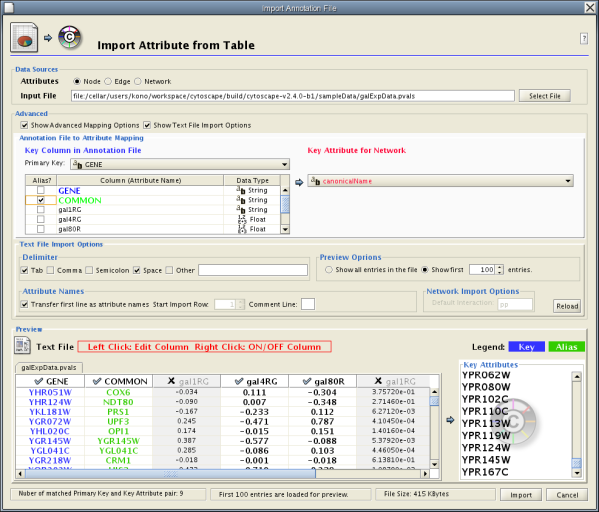
\includegraphics[width=.4\textwidth]{images/attribute_table_import_main.png} }

\begin{tabular}{|c|c|c|}
\hline 
 Object& Key Alias& SGD ID\\
\hline
 AAC3 &YBR085W|ANC3& S000000289\\
 AAT2 &YLR027C|ASP5& S000004017\\
 BIK1 &YCL029C|ARM5|PAC14 &S000000534\\
 \hline 
\end{tabular}

属性表文件应该含有主键列,最少有一列属性。属性列的数量没有限制。因为默认会将数据的第一行作为属性名称,所以Alias(别名)列是可选的。当然也可以在
File$\rightarrow$Import$\rightarrow$Attribute from Table (text/MS Excel)...
的用户界面中指定每一列属性的名称。

\subsection{基本操作}
``Import Attributes from Table''窗口的用户界面跟
``Import Network from Table''窗口的界面类似. 
\begin{enumerate}
\item 选择File $\rightarrow$Import $\rightarrow$Attribute from Table (text/MS
Excel)... 
\item 从Attributes单选按钮中选择一种属性类型,Cytoscape可以导入节点、边和网络属性。
\item 选择数据文件。 点击Select File按钮,加载本地的纯文本文件或Excel(.xls)文件。在文本框中输入远程文件的URL就能加载远程文件。点击Show Text File Import Options面板中的Reload按钮能显示远程文件的预览。
\item (可选) 如果表格分割不正确,可以调整
Text File Import Options面板中的分隔符。缺省的分隔符是制表符。
对于Excel文件则不需要这一步。
\item 缺省情况下,第一列属性是主键。有必要的话可以修改。\\
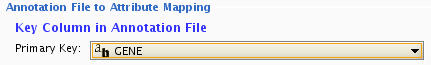
\includegraphics[width=0.3\textwidth]{images/attribute_table_import_primary_key.png} 
\item 点击Import按钮。 
\end{enumerate}
 
\subsection{高级选项}
\subsubsection{映射关键属性到主键}
以前,Cytoscape只支持节点或边名称和属性文件中主键之间的映射。在Cytoscape 2.4之后,
就没有这个限制了,通过下拉选单,不仅仅是名称,节点或边的其它各种类型的属性(字符串
、布尔、浮点数和整数)都可以作为关键属性。但暂不支持诸如列表一类的复杂属性。

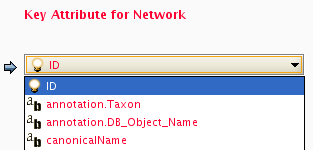
\includegraphics[width=.3\textwidth]{images/attribute_table_import_keyattr.png} 
 
\subsubsection{别名}
Cytoscape管理的别名管理机制很简单。节点和边都可以有别名。如果某个属性被设置为别名,
该属性就被视为``别名''。在映射属性时也会使用它。如果某个对象的主键和关键属性不匹配,Cytoscape就会
寻找可能匹配的别名和关键属性。在导入属性时,点击列名称左侧的选择框就能在属性表中
设置别名列。

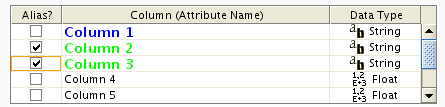
\includegraphics[width=.3\textwidth]{images/attribute_table_import_alias.png} 
 
\subsubsection{文本文件导入选项}
关于这些选项的详细信息,请阅读用户手册``创建网络''一章中的
``导入格式灵活的表格文件''。 

\subsection{属性浏览器}
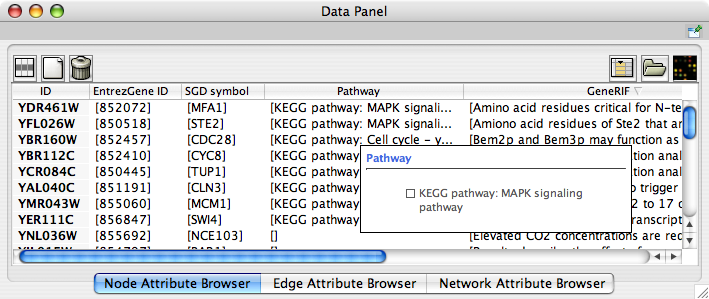
\includegraphics[width=.5\textwidth]{images/attribute_browser26.png} 
 
启动Cytoscape后,属性浏览器会出现在底部的CytoPanel中。通过F5按键或 View 
$\rightarrow$ Show/Hide attribute browser菜单项可以隐藏或显示该CytoPanel。 
跟其它的CytoPanel一样,点击其右上角的图标可以将其设为漂浮状态。

用底部面板上的``Node Attribute Browser''、``Edge Attribute Browser''和``Network
Attribute Browser''标签可以在节点、边和网络的属性之间切换。属性浏览器会显示当前
网络中所选择的节点或边的属性。选择网络中的节点或边,属性浏览器中就会出现相应的
属性信息(如图所示)。默认情况下会显示节点和边的名称。要显示其它信息,点击``Select
Attributes'' 按钮

\includegraphics[width=1em]{images/attributes_select_icon.png},然后选择所需
的属性即可(通过点击选择所需的属性,然后点击屏幕的其它地方,属性列表就会自动关闭)。
在属性浏览器中,每一列就是一个属性。双击属性单元格,可以编辑大部分属性的值;但不能编辑列表
属性和节点的ID。点击属性的表头,属性浏览器就会按字符顺序对所选择的属性的值进行排序。
点击 ``Create New Attribute''按钮

\includegraphics[width=1em]{images/attributes_new_icon.png}可以创建新的属性,但新属
性的类型只能是整数、字符串、实数(浮点)或逻辑值。用``Delete Attributes''按钮

\includegraphics[width=1em]{images/attributes_delete_icon.png}可以删除属性。
\textbf{注意:删除属性不仅会将该属性从属性浏览器中删除,还会从Cytoscape中将其删除。}
如果只是想将属性从属性浏览器中删除,点击``Select Attributes''按钮

\includegraphics[width=1em]{images/attributes_select_icon.png},取消对该属性的选择即可。

属性浏览器中的右键菜单有很多功能,比如将属性信息导出成电子表格。举个实际的例子,
点击右键菜单中的``Select All'',然后复制这些数据,就可以将其粘贴到电子表格程序中。
每个属性浏览面板中还有一个导入新属性的按钮:

\includegraphics[width=1em]{images/attributes_import_icon.png}。

节点属性面板中还有一个用于导入基因表达属性的按钮(
\includegraphics[width=1em]{images/attributes_gene_expr_icon.png} )。

\subsubsection{属性批量编辑器}
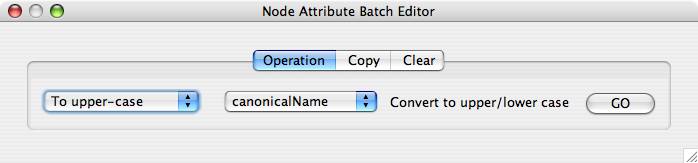
\includegraphics[width=.5\textwidth]{images/attribute_editor26.png} 

从Cytoscape 2.6开始,属性浏览器有了新的属性批量编辑器,从而实现了属性值的批量编辑。
例如,如果创建了一个名为Modules的新属性,要为每组选定的节点设置模块名称,就可以使用
批量编辑器中的Set命令。
